% Intended LaTeX compiler: pdflatex
\documentclass[a4j,12pt,openany,uplatex,dvipdfmx]{jsbook}
\usepackage[utf8]{inputenc}
\usepackage[T1]{fontenc}
\usepackage{graphicx}
\usepackage{grffile}
\usepackage{longtable}
\usepackage{wrapfig}
\usepackage{rotating}
\usepackage[normalem]{ulem}
\usepackage{amsmath}
\usepackage{textcomp}
\usepackage{amssymb}
\usepackage{capt-of}
\usepackage{hyperref}
\usepackage{coco-jsbook}
\FileVersion{1.0}
\CopyrightAuthor{島野善雄}
\CopyrightYear{2019}
\ConfidentialLevel{機密情報ではない}
\author{島野 善雄\thanks{shimano.yoshio@jp.fujitsu.com}}
\date{\today}
\title{文書作成ツールとしての Org mode}
\hypersetup{
   bookmarks=true,
   bookmarksnumbered=true,
   colorlinks=true,
   setpagesize=false,
   linkcolor=blue,
   citecolor=blue,
   backref,
   pdfauthor={島野 善雄},
   pdftitle={文書作成ツールとしての Org mode},
   pdfkeywords={Ubuntu Linux \LaTeX{}},
   pdfsubject={\LaTeX{} Tips},
   pdfcreator={Emacs 26.3 (Org mode 9.3.7)}, 
   pdflang={Ja}}
  \begin{document}

\maketitle
\setcounter{tocdepth}{4}
\tableofcontents

\listoffigures
\listoftables

\mainmatter


\chapter{はじめに}
\label{sec:orgc5ecff6}
\section{この文書の内容}
\label{sec:orgc5e82c0}
この文書では、文章作成ツールとしての Org mode の使用方法を説明します。



\chapter{Org-mode の中で図を書く}
\label{sec:orgc8b128c}

図を描くのではなく、図をテキストで書きます。



\section{blockdig を使ったダイアグラムの作成}
\label{sec:orgde8a648}
\index{blockdig}

\subsection{blockdig 参考文献}
\label{sec:org42f7b09}



\subsection{blockdig のインストール}
\label{sec:org57e2fd4}

\begin{programlist}[label={code: install-blockdiag}]{shell}{: blockdig のインストール}pip instal blockdiag reportlab 
\end{programlist}



\subsection{blockdiag の例}
\label{sec:org731ae03}



\begin{programlist}[label={code:block-diagram-w-blockdiag-1}]{text}{: }blockdiag {
  // ノードのメトリックスの設定
  node_width = 200;  // デフォルト値は 128
  node_height = 100;  // デフォルト値は 40

  // Set span metrix
  span_width = 240;  // default value is 64
  span_height = 120;  // default value is 40

  // set default shape
  default_shape = roundedbox;  // default value is 'box'

  // デフォルトの色の設定
  default_node_color = lightblue;
  default_group_color = "#7777FF";
  default_linecolor = blue;
  default_textcolor = red;

  甲 -> 乙 [label = "Use long long\nedge label"];
  甲 -> 丙;

  group {
    丙;
  }
}
\end{programlist}

\begin{center}
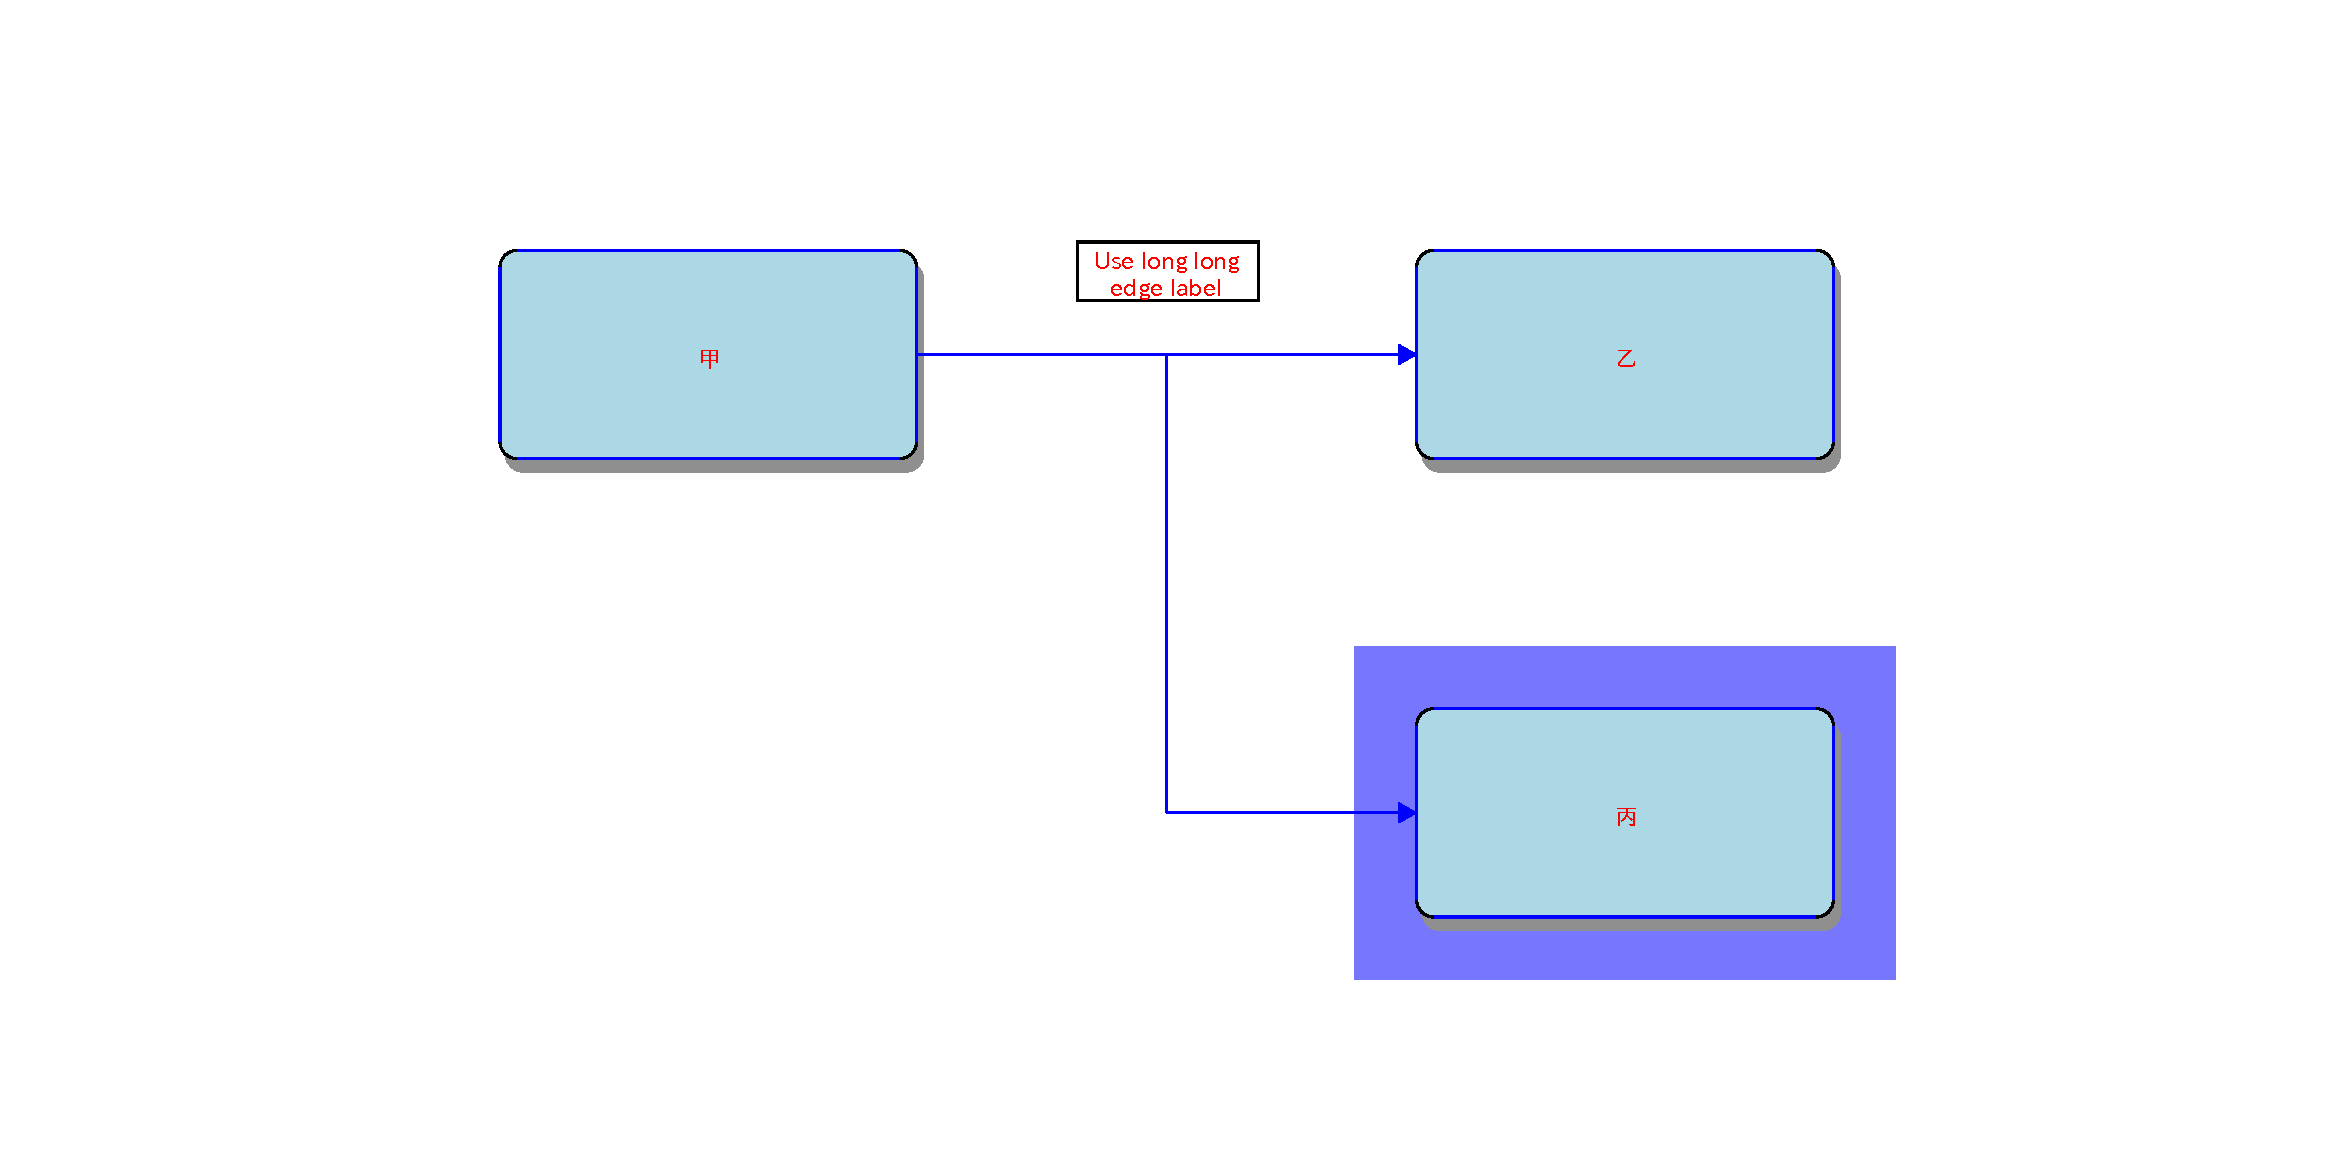
\includegraphics[width=.7\linewidth]{figs/blockdiag1_1.pdf}
\end{center}

\begin{programlist}[label={code:block-diagram-w-blockdiag-1-svg}]{text}{: }blockdiag {
  // ノードのメトリックスの設定
  node_width = 200;  // デフォルト値は 128
  node_height = 100;  // デフォルト値は 40

  // Set span metrix
  span_width = 240;  // default value is 64
  span_height = 120;  // default value is 40

  // set default shape
  default_shape = roundedbox;  // default value is 'box'

  // デフォルトの色の設定
  default_node_color = lightblue;
  default_group_color = "#7777FF";
  default_linecolor = blue;
  default_textcolor = red;

  甲 -> 乙 [label = "Use long long\nedge label"];
  甲 -> 丙;

  group {
    丙;
  }
}
\end{programlist}

\begin{center}
\includesvg[width=.7\linewidth]{figs/blockdiag1_1-svg}
\end{center}





\subsection{nwdiag の例}
\label{sec:orge81b9bf}



\begin{programlist}[label={code:network-diagram-w-blockdiag-1}]{text}{: blockdig を使ったネットワーク図}nwdiag {
    network FJWAN {
        gateway [address = "10.37.138.1"];
    }
    network Subnet-5F {
        address = "10.37.138.0/24"

        gateway [address = ".1"];
        wathcer [address = ".120"];
        gitlab [address = ".82"];
        ansible [address = ".56"];
        tomcat1 [address = ".60"];
        }
    network natnetwork {
        address = "10.0.2.0/24"

        wathcer [address = ".101"];
        gitlab [address = ".102"];
        ansible [address = ".103"];
        tomcat1 [address = ".104"];
    }

}
\end{programlist}

\begin{figure}[htbp]
\centering
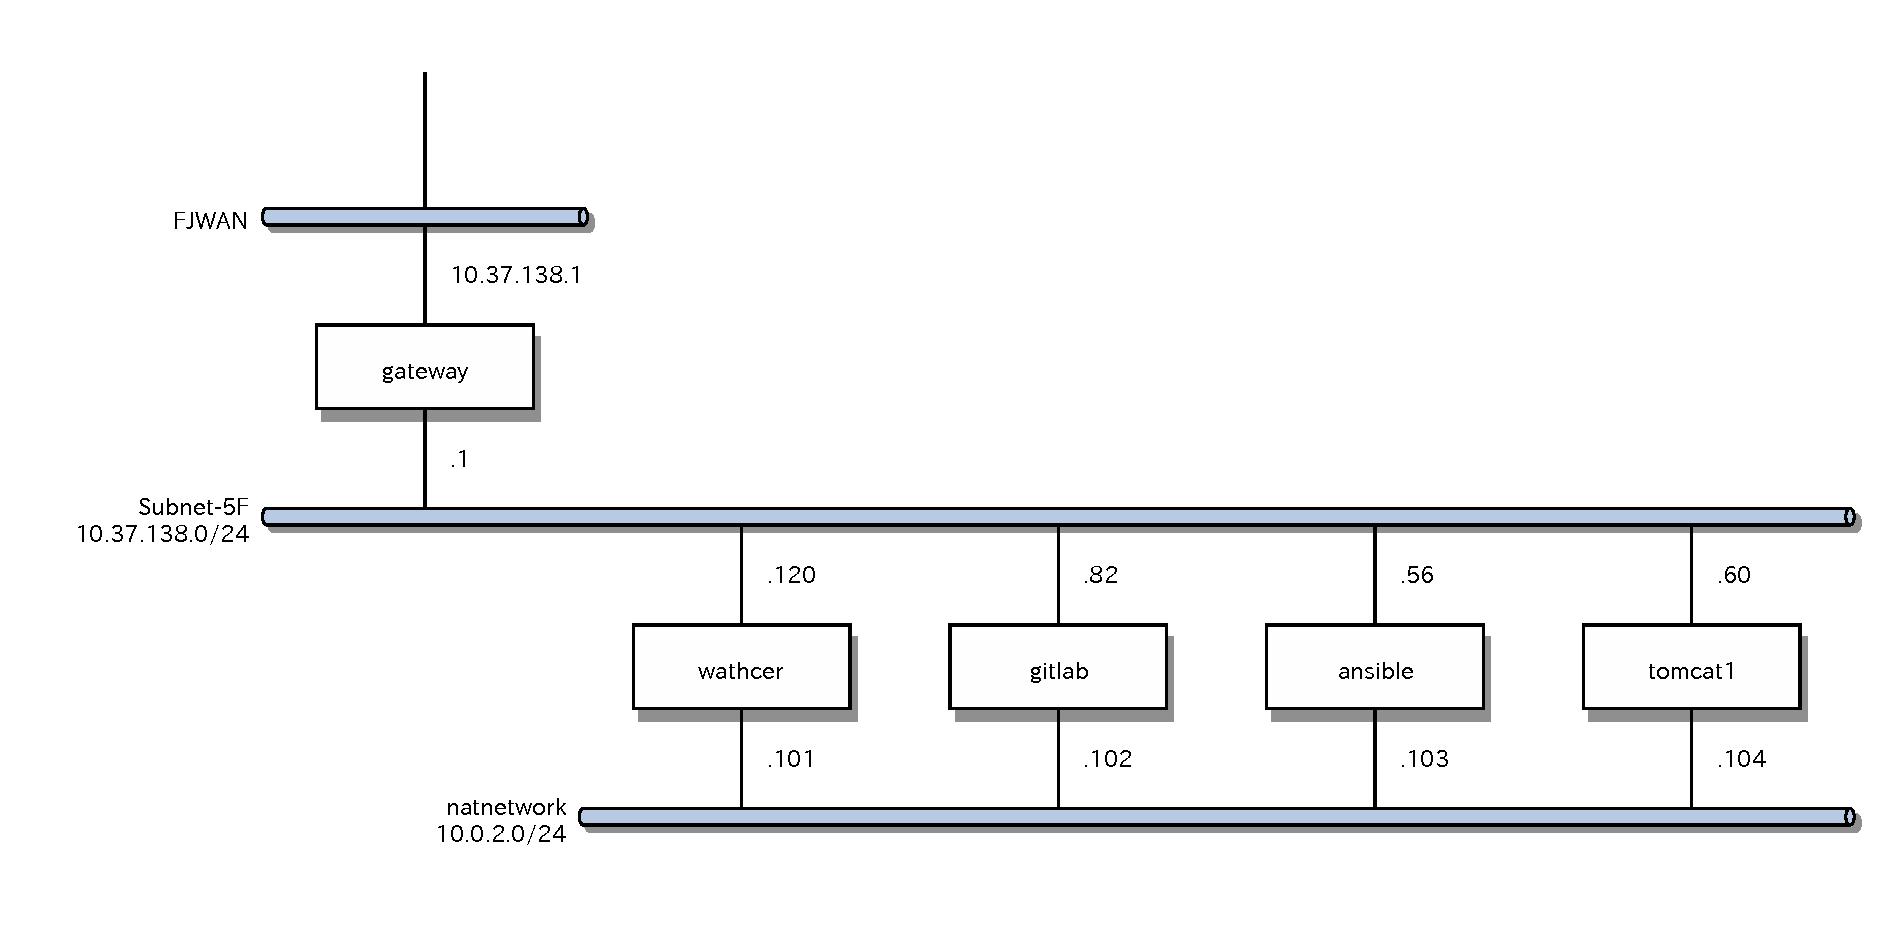
\includegraphics[width=.7\linewidth]{figs/nwdiag_1.pdf}
\caption{\label{fig:network-diagram-w-blockdiag-1}blockdig を使ったネットワーク図}
\end{figure}





\section{PlantUML を使う}
\label{sec:org2a06530}

sudo apt install graphviz

\begin{itemize}
\item \href{https://plantuml.com/ja/}{シンプルなテキストファイルで UML が書ける、オープンソースのツール}
\end{itemize}


\begin{center}
\includesvg[width=.7\linewidth]{figs/plantuml-animal}
\end{center}


\chapter{Org mode から \LaTeX へのエクスポート}
\label{sec:org3b2651c}
\index{\LaTeX}



\section{Org mode  \LaTeX{} エクスポート参考文献}
\label{sec:org1d54f5d}
\begin{itemize}
\item \href{https://emacs.stackexchange.com/questions/26179/change-org-mode-table-style-just-for-latex-export}{Change org-mode table style just for \LaTeX{} export - Emacs Stack Exchange}
\item \href{https://stackoverflow.com/questions/50573322/org-mode-how-to-use-custom-command-when-exporting-figures}{emacs - org-mode how to use custom command when exporting figures - Stack Overflow}
\item \href{https://tex.stackexchange.com/questions/348286/org-mode-latex-pdf-centering-side-by-side-images}{graphics - Org-mode, \LaTeX{}, PDF \& centering side by side images - \TeX{} - \LaTeX{} Stack Exchange}
\end{itemize}


\chapter{Org mode を使ったブログの作成}
\label{sec:org7183907}
\chapter{Org mode から HTML へのエクスポート}
\label{sec:org05cfc30}
\index{HTML}


\chapter{org-ref を使った参考文献管理}
\label{sec:orgd1ba470}
\begin{itemize}
\item \href{https://org-technology.com/posts/org-ref.html}{Emacs の org-ref で文献参照・相互参照のリンクを挿入する | org-技術}
\item \href{https://github.com/jkitchin/org-ref}{jkitchin/org-ref: org-mode modules for citations, cross-references, bibliographies in org-mode and useful bibtex tools to go with it.}
\end{itemize}


\chapter{Bittex の参考文献のあつめかた}
\label{sec:org87fd7b7}
\section{Amazon から Bibtex エントリへ}
\label{sec:orgfd55f4a}
\begin{itemize}
\item \href{http://lead.to/amazon/jp/search/use.htm}{Amazon のカスタマイズ検索(Lead2Amazon)}
\item \href{http://lead.to/amazon/jp/}{Lead2Amazon:日本語}
\end{itemize}

\section{Web から Bibtex エントリへ}
\label{sec:orgeb662c9}
\begin{itemize}
\item \href{https://chrome.google.com/webstore/detail/bibtex-entry-from-url/mgpmgkhhbjgkpnanlmlhibjfgpdpgjec}{BibTeX entry from URL - Chrome ウェブストア}
\end{itemize}


表示中の Web ページを Bibtex エントリに変換してくれます

@misc{BibTeXen88:online,
author = {},
title = {BibTeX entry from URL - Chrome ウェブストア},
howpublished = {\url{https://chrome.google.com/webstore/detail/bibtex-entry-from-url/mgpmgkhhbjgkpnanlmlhibjfgpdpgjec}},
month = {},
year = {},
note = {(Accessed on 03/11/2019)}
}

\chapter{Org mode から Microsoft Word へのエクスポート}
\label{sec:org174b830}
変換には Pandoc を使います。
\begin{itemize}
\item \href{https://github.com/kawabata/ox-pandoc}{GitHub - kawabata/ox-pandoc: Another org-mode exporter via pandoc.}
\item \href{http://nenono.hatenablog.com/entry/2015/02/10/173516}{実務に使うプレーンテキスト→Microsoft Word 変換、あるいは Pandoc を使い始めた話 - 技術 memo}
\item \href{http://peccu.hatenablog.com/entry/2015/05/12/000000}{pandoc で利用するテンプレートを指定する(org-mode から Word(docx)ファイルを作成して Pages で開くと幸せ) - @peccul is peccu}
\item \href{https://taipapamotohus.com/post/org-mode\_paper\_4/}{Emacs の org-mode で論文を書く(その 4:pandoc を利用して org-mode から word \{docx\}を文献付きで export する) | A perfect autumn day}
\end{itemize}


\section{Pandoc のインストール}
\label{sec:orgf678483}
次のコマンドを使ってインストールします:

\begin{programlist}[label={nil}]{shell}{: }conda install pandoc
\end{programlist}



\section{テンプレート作成}
\label{sec:orgc9ec5ed}
\begin{itemize}
\item \href{https://qiita.com/sky\_y/items/5fd5c9568ea550b1d7af}{ドキュメント変換ツール Pandoc:ユーザーズガイドを熟読して分かったマニアックな使い方 - Qiita}
\item \href{https://shaunakelly.com/word/styles/modifyastyle.html}{How to modify styles in Microsoft Word | ShaunaKelly.com}
\end{itemize}


@andoc --print-default-data-file reference.docx > reference.docx
\chapter{EPUB エクスポート}
\label{sec:org4b8c273}
\begin{itemize}
\item \href{https://github.com/ofosos/ox-epub}{GitHub - ofosos/ox-epub: Org mode epub export}
\end{itemize}
\chapter{Beamer エクスポート}
\label{sec:org47f5f36}
\begin{itemize}
\item \href{https://github.com/fniessen/refcard-org-beamer}{GitHub - fniessen/refcard-org-beamer: Org Beamer reference card}
\item \href{https://ryogan.org/blog/2016/01/06/emacs-org-mode-\%25E3\%2581\%25AE-beamer-export-\%25E3\%2581\%25AB\%25E3\%2581\%25A4\%25E3\%2581\%2584\%25E3\%2581\%25A6\%25E5\%25B0\%2591\%25E3\%2581\%2597/}{Emacs Org Mode の Beamer Export について少し | 澍法雨}
\item \href{https://qiita.com/htlsne/items/70cbb488e7a87cd9e228}{\LaTeX{} Beamer の\&quot;Beamer らしく\&quot;ないおすすめテーマ集 - Qiita}
\end{itemize}





\chapter{Org mode のエクスポートの一般的な参考文献}
\label{sec:org240de17}
\begin{itemize}
\item \href{https://orgmode.org/worg/exporters/filter-markup.html}{Marking Up Elements to be Exported}
\item \href{https://orgmode.org/worg/dev/org-export-reference.html}{Org Export Reference Documentation}
\end{itemize}


\chapter{ox-epub}
\label{sec:org446cbf9}
\begin{itemize}
\item \href{https://github.com/ofosos/ox-epub}{GitHub - ofosos/ox-epub: Org mode epub export}
\end{itemize}


\chapter{\LaTeX の設定}
\label{sec:org3591550}


\section{カスタムの \LaTeX 関係のファイルを置いておく場所}
\label{sec:org23375be}

\section{dvipdfmx でヒラギノを使う}
\label{sec:orgf91feca}


mkdir -p  \textasciitilde{}/texmf/fonts/opentype/hiragino


\begin{programlist}[label={nil}]{shell}{: }ln -fs "/home/shimano/.fonts/ヒラギノ明朝 Pro W3.otf" /home/shimano/texmf/fonts/opentype/hiragino/HiraMinPro-W3.otf
ln -fs "/home/shimano/.fonts/ヒラギノ明朝 Pro W6.otf" /home/shimano/texmf/fonts/opentype/hiragino/HiraMinPro-W6.otf
ln -fs "/home/shimano/.fonts/ヒラギノ丸ゴ Pro W4.otf" /home/shimano/texmf/fonts/opentype/hiragino/HiraMaruPro-W4.otf
ln -fs "/home/shimano/.fonts/ヒラギノ角ゴ Pro W3.otf" /home/shimano/texmf/fonts/opentype/hiragino/HiraKakuPro-W3.otf
ln -fs "/home/shimano/.fonts/ヒラギノ角ゴ Pro W6.otf" /home/shimano/texmf/fonts/opentype/hiragino/HiraKakuPro-W6.otf
ln -fs "/home/shimano/.fonts/ヒラギノ角ゴ Pro W8.otf" /home/shimano/texmf/fonts/opentype/hiragino/HiraKakuPro-W8.otf
ln -fs "/home/shimano/.fonts/ヒラギノ明朝 ProN W3.otf" /home/shimano/texmf/fonts/opentype/hiragino/HiraMinProN-W3.otf
ln -fs "/home/shimano/.fonts/ヒラギノ明朝 ProN W6.otf" /home/shimano/texmf/fonts/opentype/hiragino/HiraMinProN-W6.otf
ln -fs "/home/shimano/.fonts/ヒラギノ丸ゴ ProN W4.otf" /home/shimano/texmf/fonts/opentype/hiragino/HiraMaruProN-W4.otf
ln -fs "/home/shimano/.fonts/ヒラギノ角ゴ ProN W3.otf" /home/shimano/texmf/fonts/opentype/hiragino/HiraKakuProN-W3.otf
ln -fs "/home/shimano/.fonts/ヒラギノ角ゴ ProN W6.otf" /home/shimano/texmf/fonts/opentype/hiragino/HiraKakuProN-W6.otf
ln -fs "/home/shimano/.fonts/ヒラギノ角ゴ ProN W8.otf" /home/shimano/texmf/fonts/opentype/hiragino/HiraKakuProN-W8.otf

\end{programlist}



\chapter{付録}
\label{sec:org5668ae8}
\appendix
\section{後書き}
\label{sec:org2290dd6}
後書きを書きます
\end{document}